% Created with jtex v.1.0.20
% Version 3.4 Generated 2018/06/15
%
% When submitting your files, remember to upload this *tex file, the pdf generated with it,
% the *bib file (if bibliography is not within the *tex) and all the figures.

\documentclass[utf8]{FrontiersinHarvard} % for articles in journals using the Harvard Referencing Style (Author-Date), for Frontiers Reference Styles by Journal: https://zendesk.frontiersin.org/hc/en-us/articles/360017860337-Frontiers-Reference-Styles-by-Journal
% \documentclass[utf8]{FrontiersinVancouver} % for articles in journals using the Vancouver Reference Style (Numbered), for Frontiers Reference Styles by Journal: https://zendesk.frontiersin.org/hc/en-us/articles/360017860337-Frontiers-Reference-Styles-by-Journal
% \documentclass[utf8]{frontiersinFPHY_FAMS} % Vancouver Reference Style (Numbered) for articles in the journals "Frontiers in Physics" and "Frontiers in Applied Mathematics and Statistics"

%\setcitestyle{square} % for articles in the journals "Frontiers in Physics" and "Frontiers in Applied Mathematics and Statistics"
\usepackage{url,hyperref,lineno,microtype,subcaption}
\usepackage[onehalfspacing]{setspace}



% \linenumbers

\def\keyFont{\fontsize{8}{11}\helveticabold}
%% \def\Authors{First Author\,$^{1,*}$, Co-Author\,$^{2}$ and Co-Author\,$^{1,2}$}
\def\firstAuthorLast{Nathan Cashion} %use et al only if is more than 1 author
\def\Authors{Nathan Cashion\,$^{}$}
% Affiliations should be keyed to the author's name with superscript numbers and be listed as follows: Laboratory, Institute, Department, Organization, City, State abbreviation (USA, Canada, Australia), and Country (without detailed address information such as city zip codes or street names).
% If one of the authors has a change of address, list the new address below the correspondence details using a superscript symbol and use the same symbol to indicate the author in the author list.
\def\Address{}
% The Corresponding Author should be marked with an asterisk
% Provide the exact contact address (this time including street name and city zip code) and email of the corresponding author

\begin{document}
\onecolumn
\firstpage{1}

\title[]{Advancing Telemedicine in Musculoskeletal Practice}

\author[\firstAuthorLast ]{\Authors} %This field will be automatically populated
\address{} %This field will be automatically populated
\correspondance{} %This field will be automatically populated

% If there are more than 1 corresponding author, comment this line and uncomment the next one.
\extraAuth{}
% \extraAuth{corresponding Author2 \\ Laboratory X2, Institute X2, Department X2, Organization X2, Street X2, City X2 , State XX2 (only USA, Canada and Australia), Zip Code2, X2 Country X2, email2@uni2.edu}

\maketitle
%% Leave the Abstract empty if your article does not require one, please see the Summary Table for full details.
\begin{abstract}
\section{}
Telemedicine has rapidly emerged as a promising approach to managing back, neck, and other musculoskeletal (MSK) pain. Despite impressive advances in the technology, clinicians and patients remain reluctant to adopt it. The transition to telemedicine from hands-on, in-person care presents numerous barriers. In contrast, new technologies and tools are readily embraced by early-adopters in other industries, such as video game streaming, fitness influencers, and YouTube content creators. By adopting tools and techniques from these other industries, MSK providers may be able to increase in-session engagement and patient satisfaction with telemedicine.

\keyFont{ \section{Keywords:} telemedicine, telehealth, musculoskeletal, engagement, live streaming, video conferencing}
\end{abstract}

\begin{figure}[!htbp]
\centering
\includegraphics[width=1\linewidth]{files/tgSYYIag2qhHH1yPOHt4-6b7880ee2e054686c72c14bae4bbb156.png}
\end{figure}

\section{Introduction}

Telemedicine has the potential to bring healthcare to millions of patients who are unable to visit their doctor. This holds true even in specialties that traditionally demand a face-to-face, such as chiropractic, osteopathy, physical therapy, and pain medicine. Surprisingly, these specialties focused on musculoskeletal conditions have also benefited from the use of telemedicine, particularly during the COVID-19 pandemic \citep{lamplotGoodComesEvil2021}.

However, video calls leave much to be wanted, especially for conditions that are commonly examined and treated with direct, physical touch via physiotherapy, chiropractic, and massage. Patients and their clinicians observe feelings of disconnect during their live video calls \citep{ahmadPatientPerspectivesTelemedicine2023}. Healthcare systems and private clinics have been slow to include telemedicine in MSK practice for various reasons, including cost, resistance to change, and lack of clarity on the benefits and feasibility in this specialty \citep{daviesInternationalCoreCapability2021}. Learning how to make telemedicine a better experience for both patients and clinicians can accelerate the potential reach of this promising technology.

\subsection{Overview of Topic}

\textit{Telemedicine} is defined as the practice of caring for patients from a distance \citep{jinTelemedicineCurrentImpact2020}. \textit{Telehealth} is a broader term that can include population-based efforts in public and global health. In contrast, the focus of telemedicine is on a single patient or small group of patients \citep{barberioTransitioningTelehealthTodays2021}. \textit{Telerehabilitation} is another term that is often used interchangeably with telemedicine for musculoskeletal conditions, particularly physical therapy in post-surgical scenarios \citep{baroniStateArtTelerehabilitation2023}. While the topic of this paper is focused on musculoskeletal applications, most of the concepts do apply to other specialties. Hence, I will use telemedicine throughout for consistency.

Telemedicine has been used in various forms for centuries (consider carrier pigeons being used to suggest tinctures for the plague or phone calls to the family doctor for a child's late-night stomachache) \citep{jinTelemedicineCurrentImpact2020}. Modernly, it has become nearly synonymous with implementations via the internet, such as video conferencing calls between a provider and a patient \citep{daviesInternationalCoreCapability2021}.

Telemedicine offers many benefits to patients, but legislation has not kept up with demand. As a result of the pandemic, legislation required insurance companies to pay for telemedicine visits with temporary exceptions allowing for greater access across state lines \citep{barberioTransitioningTelehealthTodays2021}. However, while some aspects of this have been extended, it is unclear whether reimbursement will continue for all services across all specialties \citep{TelehealthHereStay2021}. For telehealth to have a positive effect on healthcare, several challenges must be addressed in policy and research.

\subsection{Identification of Gap}

Beyond the slow adjustments in legislation and reimbursements, telemedicine has suffered in hasty roll-outs that have not afforded optimal infrastructure or training to take place. In fact, one of the key factors in clinicians' reluctance to use telehealth is the lack of familiarity with the technology and ideal procedures for conducting virtual visits with patients \citep{daviesInternationalCoreCapability2021}.

While most of us were forced to rapidly adapt to a Zoom-centered culture, using the same tools for different situations can lead to sub-optimal experiences. A conversation about low back pain, for example, is meant to be a dynamic collaboration between patient and provider, often including the use of visuals such as physical anatomical models to illustrate the underlying structures that may be associated with pain syndromes. Experiences like these are challenging to achieve in a 2-dimensional, relatively static video call when both participants are limited to showing themselves from the mid-torso to above the head. Even worse, Zoom meetings are often affected by quality issues such as poor-audio or bad lighting that make it difficult for the participants to understand one another, let alone forge an emotional connection. Problems with internet connectivity can interrupt a speaker mid-sentence or prevent a call from starting altogether.

Advances in audio and video technology, however, make it possible for amateurs and hobbyists to create high-quality video content, including well-produced, livestreaming video. Fitness influencers post ultra-high definition videos to educate and entertain their followers about healthcare topics on social media and YouTube. From the average bedroom -- or their parents' basement -- `gamers' broadcast their video game activities to hundreds of thousands of engaged fans, using tools to create a dynamic and highly-produced experience that leaves viewers feeling like they are a part of a community.

Based on my review of the literature, there is little to no discussion about improving the technical aspects of synchronous telemedicine video calls and how they influence the patient and clinician experience. Pulling from the literature on user experience design, live video streaming, and incorporating skills from audio and video engineering, it is possible to greatly improve the experience and satisfaction of all involved.

\section{Background}

\subsection{Selection of Topic}

As a chiropractor with a passion for technology, I have been fascinated by the possibilities of providing spine care remotely, both via telemedicine or asynchronous media such as mobile apps and tools using artificial intelligence. Spurred on by the COVID-19 pandemic, telemedicine has become more common throughout all specialties, including for musculoskeletal conditions normally treated by chiropractors and physiotherapists \citep{lamplotGoodComesEvil2021}. However, due to the hands-on nature of manual therapy offered as treatment for musculoskeletal aches and pains, patients and providers have expressed doubts as to the practicality of telemedicine \citep{Barton2022It}. While physical therapies are prominent, other components of evidence-based musculoskeletal care include education and exercise prescription, both of which can be provided effectively via telemedicine solutions \citep{baroniStateArtTelerehabilitation2023}.

Patients who opt for telemedicine visits have reported positive outcomes, even if they were initially skeptical \citep{Hinman2024Telerehabilitation, Lawford2018I}. According to \citet{ernstzenYouMustUnderstand2022}, patients experiencing chronic pain who joined a group exercise program found that it helped them feel empowered. Multiple studies have determined that for patients with musculoskeletal disorders, telemedicine is as safe and effective as in-person care \citep{Bargeri2024Effectiveness, Seron2021Effectiveness, withersRemotelyDeliveredPhysiotherapy2024}.

Despite this early success, many barriers still exist that prevent more widespread adoption of telemedicine. Using a qualitative approach, \citet{wadeClinicianAcceptanceKey2014} concluded that clinician acceptance is the leading factor limiting adoption of telemedicine, followed by patient acceptance. This reluctance is reflected in the previous findings that remotely delivered care does not meet the patient's expectation of hands-on touch \citep{baroniStateArtTelerehabilitation2023}. \citet{saragiottoCanYouBe2022} commented on this paradox of being a manual therapist but not using your hands. While they found the existing literature on telemedicine was limited, the available evidence suggests that practitioners of manual therapies are able to have a positive effect on reducing pain and improving function in patients with musculoskeletal conditions in a virtual setting. Therefore, the authors recommended that manual therapists include telemedicine in their available options for treatment.

Other criteria for resistance to telemedicine include a lack of familiarity with the technology, referred to as \textit{digital literacy} \citep{fernandesWhatExtentCan2021, Manganello2017Relationship}, and the ability to build rapport and develop a therapeutic alliance between patient and practitioner \citep{wallaceGroupIndividualTelehealth2022}.

This final point has captured my attention and imagination. What is it about the experience on video calls that has people feeling disconnected? What are the elements that lead to the so-called ``Zoom fatigue'' so many of us have experienced during the rapid shift to virtual communication during the pandemic \citep{bailensonNonverbalOverloadTheoretical2021}? Are there solutions that are already being used in other industries to increase the feeling of connectedness and engagement during telemedicine appointments?

Most research to date has evaluated the presence of telemedicine in care settings as well as the results in terms of patient outcomes and safety. But have researchers considered that \textit{how} telemedicine visits are conducted may have an impact on the outcomes? In most other areas of technology, immense effort and millions of dollars are spent on refining the user-experience (UX) of digital tools and software to increase user satisfaction \citep{monachelliDesigningMHealthApps2024}. What changes could be made to the UX of telemedicine to increase patient satisfaction and decrease clinician burden?

\subsection{Literature Search}

I conducted a series of searches using EBSCOHost. A broad search for ``telehealth'' returned 180,725 results. Adding the terms ``telemedicine OR telehealth OR telerehab*'' reduced my results to 800+. I further limited the search to relevant papers using the term ``musculoskeletal''. As technology is a rapidly advancing field, I limited the Publication Date to between 2019-2024. Source types were restricted to Academic Journals and Reviews.

Searches for ``telehealth AND engagement'' provided limited results relevant to the current topic. I conducted further searches via PubMed on engagement in live streaming applications, such as video games and ecommerce with the terms ``live streaming AND engagement''. Results were varied and I narrowed the selection by scanning titles and abstracts for relevance, then reviewing related papers and papers cited by or citing the current paper.

I included other articles found via Google Scholar and Google Search that were relevant. Though they may not be peer-reviewed, they are authored by industry experts.

When new topics or keywords appeared frequently in my initial results, I explored them further by searching the same databases. I also used artificial intelligence research assistants (\href{http://Elicit.com}{Elicit.com}, \href{https://researchrabbit.ai}{ResearchRabbit.ai}) to suggest other articles or related topics.

\subsection{Literature Review}

My literature brought together research in two broad areas---the use of telemedicine in musculoskeletal health and the psychology of engagement in live-streaming video.

A review of the existing literature on telemedicine in musculoskeletal care revealed a number of themes. The majority of the research addressed trends in the use of telemedicine broadly. This thread of the literature included prevalence of remote therapies as well as acceptance and perceptions by both clinicians and patients. The second most common theme in the research concerned the reliability of the examination and diagnosis of musculoskeletal disorders via telemedicine as well as the effectiveness of treatment. Other themes included the core competencies suggested for clinicians to conduct telemedicine visits and the limitations of telemedicine in practice.

\subsubsection{Telemedicine in MSK care}

\paragraph{\textit{Trends in use and acceptance of telemedicine}}

Out of necessity, the use of telemedicine accelerated during the global COVID pandemic. A Nature Medicine editorial reflects on the trajectory of telehealth during the COVID-19 pandemic \citep{TelehealthHereStay2021}. According to Medicare data, telehealth visits increased ten-fold in a 12-month period (from March 2020--March 2021).

Telemedicine is not only used for individuals. Several programs have explored adapting group programs for chronic pain to a virtual setting. \citet{wallaceGroupIndividualTelehealth2022} conducted a scoping review of group and individual telehealth for chronic musculoskeletal pain to explore patient perspectives on virtually delivered pain management programs. From 10 included studies, the authors extracted 4 themes: usability of the technology, tailored care, therapeutic alliance, and managing behavior. The authors determined that telehealth for chronic musculoskeletal pain is acceptable by patients. Group telehealth programs additionally offer opportunities for social support and validation of the pain experience. Patients felt empowered and intrinsically motivated to modify their behavior. The authors discussed how clinicians can help develop a therapeutic alliance during telehealth interventions. This is more readily accomplished via synchronous video-conferencing rather than asynchronous messaging.

South Africa offers a group Patient Education Empowerment Programme (PEEP) for patients living with chronic pain. Due to the pandemic, this program was adapted to be delivered remotely via synchronous (group calls) and asynchronous (educational materials) methods. \citet{ernstzenYouMustUnderstand2022} interviewed six women who participated in this 6-week telehealth group program to learn what worked and what didn't. The patients felt that the program helped them start on a journey of self-discovery and personal development. Connecting with other patients experiencing similar pain and disability helped validate their experiences and motivated them to alter their behaviors. Participants reported that this method of delivering a group program for chronic musculoskeletal pain was feasible and that they felt engaged and supported. Facilitators were able to develop a therapeutic alliance through virtual communication without meeting patients in person. While there were barriers to comfortably participating in this course, facilitators were able to address them with planning. For example, data packages were provided to patients to cover the cost of increased cellular data usage.

\citet{ahmadPatientPerspectivesTelemedicine2023} surveyed nearly 500 patients who had received telemedicine care for hand surgery consultation during the pandemic. The majority of respondents liked their experience of a teleconsultation and felt satisfied with the attention received from their provider. Despite this, over two-thirds of the patients said they would still prefer an in-person visits when available. Common reasons for this choice included difficulty explaining their symptoms and the need for an in-person follow-up visit to move forward with their care.

\paragraph{\textit{Diagnosis and management of MSK conditions via telemedicine}}

\citet{ohAgreementConcurrentValidity2024} reviewed 9 studies on the assessment and management of people with MSK conditions. They found that inter-rater reliability for diagnosis involving the low back, knee, shoulder, lower limb, ankle, elbow, and shoulder was high. The authors concluded that telehealth is a feasible option for assessment of musculoskeletal conditions.

\citet{satinVirtualSpineExamination2021} provided a narrative review on how clinicians can conduct physical examination for spine-related disorders via virtual calls. The authors presented strategies for overcoming some of the difficulties unique to virtual examination of the spine.

A systematic review from \citet{bernhardssonDigitalPhysiotherapyAssessment2023}, compared face-to-face physiotherapy assessment of musculoskeletal disorders with convential assessment. Digital physiotherapy assessment was found to have moderate to almost perfect validity when compared to traditional physical exams. The authors explained that while patients thought an in-person assessment was better, they were satisfied with their experience. The reported outcomes also demonstrated excellent reliability of patient-reported outcome measures.

A study in India showed that telerehabilitation for spine pain reduced pain and disability better than standard in-clinic rehabilitation during the COVID pandemic \citep{shahEfficacyTelerehabilitationSpine2024}. As reported by \citet{barberioTransitioningTelehealthTodays2021}, an overview of clinical outcomes and patient satisfaction concluded that telemedicine offered equal or better results than usual care.

\paragraph{\textit{Core competencies for telemedicine in MSK}}

\citet{daviesInternationalCoreCapability2021} conducted a modified Delphi survey ith experts in physiotherapy, including researchers, clinicians, consumers, and representatives of physiotherapy organizations. The panel developed a framework to outline the skills and capabilities needed to deliver care via video calls. The recommendations consisted of legal and ethical topics such as patient privacy \& safety, record keeping, and licensure. The panel also outlined technical skills such as camera placement, software selection, and adapting the physical exam to a virtual setting.

\citet{haldemanDistanceManagementSpinal2021} describe the process of developing a pair of guides to help clinicians and patients manage spinal pain during the COVID-19 pandemic or in any situation that requires management from a distance. A group of 29 individuals from 10 countries including experienced clinicians, researchers, and educators collaborated through an iterative process to create two guides. The \textit{Patient Guide} includes 2 steps to help patients self-assess the severity and nature of their spinal pain and determine an appropriate course of action, such as emergency care, urgent care, or non-urgent communication with a healthcare provider. The \textit{Clinician Guide} provides a framework for providers to systematically assess and classify patient's spinal disorders. The authors suggest that telehealth visits will provide a helpful method for patients and clinicians to evaluate and manage spinal disorders when face-to-face visits are not available.

\paragraph{\textit{Limitations of telemedicine}}

As telehealth becomes more popular and widespread, it is important to recognize the strengths and weaknesses of this new platform. While many clinicians and patients see the lack of hands-on care as a drawback \citep{bartonItsSecondBest2022}, manual therapy is just one of many modalities that clinicians can use to manage patients with musculoskeletal conditions. Nevertheless, while physical touch isn't required in medicine, it is still appropriate to consider the inherent value in skin-to-skin contact.

\citet{apathyTelemedicineInPersonVisit2024} recognize that providers offering telemedicine must change their workflow. The authors analyzed how much time clinicians in a large multi-specialty clinic spent on their EHR in two types of visits -- telemedicine and standard, in-person visits. The goal was to identify whether offering telemedicine visits changed the amount of time spent on EHR documentation.

The authors found that on days with telemedicine visits, clinicians spent an average of 14.8 minutes more on documentation in the EHR compared to days with no telemedicine visits. However, on days with only telemedicine visits, there was no increase in time spent in the EHR. This suggests that mixing in-person and telemedicine visits in the clinic may lead to inefficiencies as opposed to dedicating certain days to telemedicine visits. This suggests that a hybrid approach has drawbacks. If clinicians dedicate time to telemedicine, they may see improved outcomes.

\subsubsection{Engagement in a virtual setting}

Most of the research concerning engagement in telemedicine refers to the long-term involvement of patients in their own care \citep{Lyles2020Using, monachelliDesigningMHealthApps2024}. Little research has evaluated the ways in which telemedicine providers can increase real-time engagement and satisfaction of their patients during synchronous calls. However, relevant literature exists in other applications of virtual live streaming such as e-commerce and gaming. The second part of my literature review addressed research exploring engagement and feelings of connection between live-streamers and their audience.

\paragraph{\textit{Application of intimacy theory}}

\citet{liuHowCanLive2021} examined viewer engagement in ecommerce streaming, where a presenter reviews or discusses products with a goal to sell to their audience. The authors promote \textit{intimacy theory}---the idea that acting in an authentic and transparent manner builds trust and intimacy---as a model for engaging live viewers. Several suggestions are offered. Live streamers should:

\begin{itemize}
\item respond quickly to viewers comments or questions
\item present a consistent and authentic personal brand
\item demonstrate attitudinal similarity by mirroring viewer's beliefs or opinions
\item speak directly to viewers
\item simulate direct eye contact by looking directly into the camera.
\end{itemize}

\citet{baroniStateArtTelerehabilitation2023} emphasized this last point stating that communication is the most powerful tool for clinicians to use in telemedicine consults. Looking directly into the camera helps establish an emotional connection and build trust.

\begin{figure}[!htbp]
\centering

\includegraphics[width=0.7\linewidth]{files/tgSYYIag2qhHH1yPOHt4-8051cc119966c3d24ece6c3c215db7c8.png}
\caption[]{Looking directly into the camera can simulate eye contact and help build professional intimacy}
\label{bD1TUn2aPV}
\end{figure}

\citet{lvHowLiveStreaming2022} examined factors that lead to sustained engagement by viewers of live streaming media. The authors hypothesized that there is a link between visual stimuli (such as emojis), perceived trust, and presenter's social warmth and continued viewing. The authors developed a questionnaire that received 240 responses to validate their hypotheses. Based on their findings, the authors recommend live-streaming presenters engage their audience in real-time and build long-term trust by answering questions, designing visual stimuli to support engagement, and demonstrating social warmth.

\begin{figure}[!htbp]
\centering
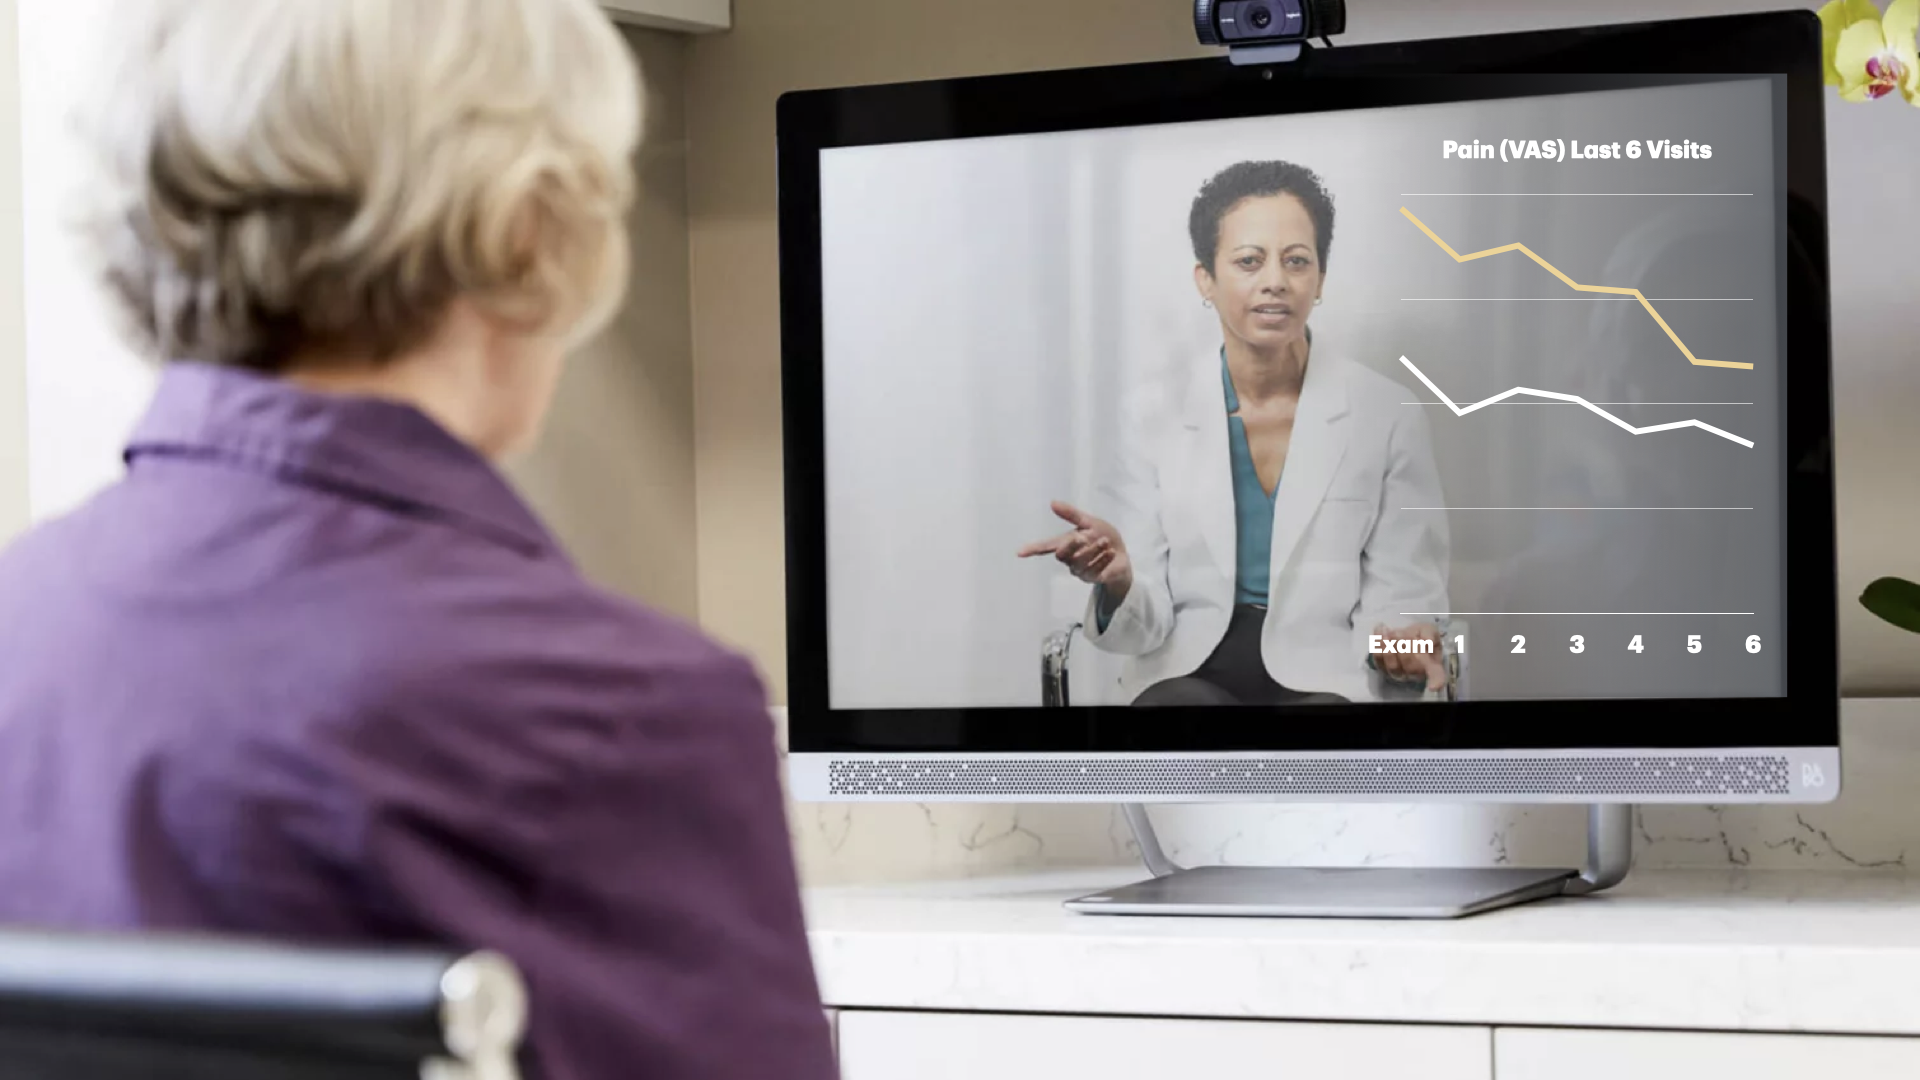
\includegraphics[width=0.7\linewidth]{files/tgSYYIag2qhHH1yPOHt4-e4b6540943de5e6953f3e889c3ee3358.png}
\caption[]{By incorporating visual stimuli, telemedicine providers can increase patient engagement.}
\label{SK3YTBY2uG}
\end{figure}

In their JAMA viewpoint, \citet{Mangione2024Out} reflect on the power of touch that has become increasingly absent in medicine. Amongst the various empirical benefits such as improved immune response, lower blood pressure, oxytocin and endorphin release, the author highlights the simple recognition that patients appreciate touch. Mangione et al. observe that along with physical touch, eye contact has also decreased in the exam room (this is not a necessary casualty of telehealth---providers can simulate eye contact by learning to look directly into the camera).

\paragraph{\textit{Content quality}}

\citet{liImpactFitnessInfluencers2023} examined how the characteristics of fitness influencers impacted people's perceived connection and behaviors. The authors found that personal attributes, such as attractiveness, and the quality of content were associated with viewers' motivations to exercise. By presenting high quality content and engaging with their viewers, social media influencers facilitated parasocial relationships which positively influence their viewers' behaviors. This research suggests that content quality is an important factor in achieving desired results from viewers.

\begin{figure}[!htbp]
\centering
\includegraphics[width=0.7\linewidth]{files/tgSYYIag2qhHH1yPOHt4-de7f7acb347f1ab4852167e620469c97.png}
\caption[]{YouTubers like \href{https://youtube.com/@cleoabram}{Cleo Abram} focus on content quality over quantity, resulting in high viewer engagement.}
\label{ClmRhKctf5}
\end{figure}

\section{Problem}

Most of us were forced to get comfortable with remote work and virtual conferencing during the pandemic. After an initial learning curve, people began recognizing the myriad benefits of not having to go into the office such as avoiding traffic, increased productivity, and the convenience of flexible schedules \citep{mollaTellYourBoss2022, tsipurskyUnlockingRemoteWork2023}. But as more time passed, those benefits lost their novelty and people began noticing negative effects, often referred to as \textit{Zoom fatigue} \citep{bailensonNonverbalOverloadTheoretical2021}. Many companies made the controversial call to return to the office.

A similar pattern is emerging with the prevalence of telemedicine visits. According to data from the National Center for Health Statistics, the percentage of people who used telemedicine visits declined by 7\% from 2021 to 2022, after a dramatic rise in the early pandemic \citep{lucasDeclinesTelemedicineUse2024}.

But what if these negative effects of remote work and video conferencing were not inherent to the tools, but attributable to user error? \citet{lindsayAddressingZoomFatigue2021}, an expert in live streaming media, discussed the common perception of Zoom fatigue and why he considers it a misconception. He argues that by learning some basic skills familiar to those in the broadcast industry, online conferencing does not necessarily lead to disconnect. Rather, by embracing a virtual-first approach and acquiring readily available tools, connecting over video-conferencing can actually feel more authentic and personal. A similar mechanism may explain the subpar experience as the world has transitioned to more frequent telemedicine video calls.

\citet{lindsayHowProduceGreat2019a}, also reflects on another technology transition to illustrate the current limitations in video broadcasting. When motion pictures were first produced in theaters, they were essentially films of stage plays. Over the decades, filmmakers realized they were not constrained by the physical stage and began using different techniques to push the technology further. Cinema today looks nothing like those first motion pictures, which Lindsay calls quaint. Similarly, conducting telemedicine visits in the same way we take business calls over Zoom is quaint. There is so much more the technology can offer us and we don't need to be constrained by old formats.

For most providers, telemedicine is a secondary option -- a backup for when an in-person visit is unavailable or the patient is too far away. They try to do everything they would in a normal visit, but confine themselves to a laptop screen and standard Zoom call. If they're feeling adventurous, they might try a screenshare, but usually they'll just talk while looking at the patient's chart in an EMR next to -- or even in front of -- the video window.

This approach might work fine for some specialties. Routine visits with a primary care provider to review lab results, for example, or a 6 month post-op check-in with a surgeoun don't require much more than a chat. But other specialties that involve a more hands-on approach and the need to see whole-body movement leave a lot to be desired \citep{bartonItsSecondBest2022}.

What if we could rethink the virtual visit and re-imagine it with fresh eyes? Instead of simply inserting the Zoom window into an existing clinical workflow, what if we built a new encounter around the tools currently available for connecting with people from afar?

Companies are attempting to create advanced methods of providing telemedicine such as the Holobox which recreates a full-body 3D projection of the caller \citep{TelehealthHolograms2023}. But these solutions are impractical and out of reach for the average clinician and patient at the present moment. Other innovators are turning to virtual reality headsets, like the Apple Vision Pro \citep{sissonApplesNewVision2024}. But these devices are still clunky and create a completely different paradigm than what patients and providers are used to.

Another approach to managing musculoskeletal conditions from a distance involves removing the clinician from the synchronous interaction. \citet{weiOnDemandVirtualPhysical2019} proposed a novel virtual physical therapist system for patients with Parkinson's disease. By using Microsoft Kinect sensors and machine learning algorithms, rehabilitation exercises can be monitored and adjusted by an application with occasional review by a physical therapist. In a similar way, Sword Health, a digital physical therapy provider, provides AI-augmented care plans and motion sensors to treat musculoskeletal (MSK) conditions \citep{herzlingerSwordHealth2022}. While such innovations are promising, they are so far outside of the current healthcare delivery paradigm that they are unlikely to be readily adopted by current healthcare systems.

These initiatives demonstrate, however, that to make progress in healthcare, it is often helpful to look to outsiders who can reframe the problem \citep{khoslaventuresWinningOutsiderBuilding2023, staeritzHowCanHealthcare2021}. Let's look to another industry that has made live, synchronous video engaging and popular -- video game streaming.

Gamers use off-the shelf video and audio gear together with free, open-source software to produce high-definition, engaging live-streams from their bedroom. According to StreamYard \citep{HowMuchMoney2023}, these productions draw millions of viewers and earn top streamers a healthy six-figure monthly income. This prompts the question:

\paragraph{\textbf{What can telemedicine providers learn from live streamers?}}

The current research on telemedicine shows it is a viable alternative for most of what occurs during regular visits. Gathering the patient's subjective complaints, conducting a history, performing a comprehensive exam, determining a likely diagnosis and prognosis, and providing patient education can all be done as well or better than in-person for many conditions, including spine pain \citep{ansaryVirtualPhysicalExam2021, satinVirtualSpineExamination2021}.

Qualitative research on telemedicine offerings reveal generally positive feedback from patients and clinicians with the occasional mention of barriers to access or problems with connection \citep{ahmadPatientPerspectivesTelemedicine2023, hinmanSoundsBitCrazy2017}. More guidelines are offering suggestions for including telemedicine in medical education curriculum \citep{daviesInternationalCoreCapability2021}. However, these consensuses are limited to basic concepts of patient safety, privacy, and basic digital literacy -- all important, but insufficient to make significant improvements beyond the status quo.

\section{Plan}

Telemedicine has proven to be a valuable component to evidence-based musculoskeletal care. However, barriers exist that limit the reach of this valuable tool. By addressing the perception that telemedicine is inferior to in-person visits as well as the real-time experience during video calls, this research may help to persuade more providers to adopt telemedicine as a viable means to providing education and guidance to people in pain.

In addition to training musculoskeletal clinicians on core competencies related to telemedicine, additional training should be offered on advanced topics, such as intimacy theory to develop a strong therapeutic alliance and the software and tools to enhance the user-experience.

The group fitness app Peloton is an example of what well-produced telemedicine can aspire to. Professional instructors guide a live or virtual group of cyclists through a pre-planned workout that is broadcast to subscribers. A small technical crew operate the studio and use multiple camera angles to create a dynamic, choreographed performance. The instructor is trained to speak directly to an imagined participant while looking into the camera. This significant effort results in a unique, engaging experience that journalists have described as intimate, citing social media posts idolizing the celebrity instructors \citep{bryantTheresIntimacyWhat2020}.

\begin{figure}[!htbp]
\centering
\includegraphics[width=0.7\linewidth]{files/tgSYYIag2qhHH1yPOHt4-d80513f8d7552ef9ea56f39bd3e4c521.png}
\caption[]{Peloton instructors are trained to speak directly to participants while taking advantage of multiple camera angles.}
\label{zDL8HO3c8L}
\end{figure}

While Peloton is a high-end luxury fitness brand, there are elements to the production that can be applied to telemedicine. Clinicians can be trained to build a stronger connection with their patients over video calls by incorporating the elements of authenticity and looking directly into the camera. Using additional software and hardware, clinicians can choose from different camera angles that allow them to demonstrate full-body movements with side- or front-views as well as returning to a standard, close-up view when listening to or speaking to the patient. This software can also be configured to seamlessly show additional content such as radiographs that can be annotated in real-time or data-visualizations showing the patient's progress with treatment.

Virtual webcam software is one option to enhance the telemedicine experience. \href{https://obsproject.com/}{Open Broadcaster Software (OBS)} is a free and open-source cross-platform application built for video live streaming. \href{https://ecamm.com/}{eCamm Live} is a commercial alternative that offers a shorter learning curve and more refined user-interface, but is only available for macOS. Both applications have a similar feature set, including the ability to build custom `scenes' with a particular layout of video, audio, and screen sources. The operator (in this case a telemedicine provider) can switch between these scenes on the fly with the push of a button. For example, a provider can start with a simple close-up angle to open the call, switch to a full-body angle while demonstrating clinical exam procedures, then switch to a scene with both close-up video and a window capture showing a digital anatomical model of a body part of interest.

Another popular tool in live streaming is the \href{https://www.elgato.com/us/en/s/explore-stream-deck}{Elgato StreamDeck}, a small keypad with customizable buttons and software that integrates with various applications including OBS and eCamm Live. The StreamDeck can act as a hardware controller for OBS or eCamm to switch between scenes or trigger animations or other actions on the video call. Elgato also makes the Prompter, a small display with a one-way mirror that acts as a teleprompter. This---or other teleprompter devices---can be used to place the incoming video of a patient directly in front of the camera lens, making it easy for the provider to maintain eye contact throughout the call.

Combining these tools with a variety of options for additional cameras, lighting, and audio equipment can allow a provider to create a powerful telemedicine studio. Paired with clinician training to take advantage of these new tools and engage the patient effectively, this set-up can enhance the quality of telemedicine video calls.

\subsection{Key Uncertainties}

Despite the promising potential of this proposal, a few areas of uncertainty remain.

\subsubsection{Security and Confidentiality}

As previously mentioned, patient privacy and confidentiality are key concerns in healthcare, including in telemedicine. Clinical software is required to by HIPAA compliant and is often reviewed by the Federal Drug Administration \citep{jinTelemedicineCurrentImpact2020}. Programs such as OBS and eCamm Live are designed to be used in one-to-many live-streaming scenarios, which may not involve the end-to-end encryption now required of telehealth platforms. However, this broadcast function is not on by default. The app simply inserts itself in the video pipeline to act as a virtual webcam, and all processing of the video and audio data is done on-device. The software can work with HIPAA-compliant telehealth software such as Zoom or \href{http://Doxy.me}{Doxy.me}. Nevertheless, the open-source nature of these tools raises concerns about HIPAA-compliance and security that must be addressed before these recommendations are implemented.

\subsubsection{Financial and Logistic Feasibility}

Compared to professional broadcast gear, the software and devices discussed are accessible and inexpensive. Yet, they do constitute an additional expense beyond the current standard set-up for musculoskeletal telemedicine providers. The increased cost includes hardware (additional cameras, microphone, lighting, StreamDeck, etc.) and potential licensing or subscription fees for virtual webcam software. This cost can be mitigated by the use of open source software which does not require any licensing or subscription fees.

Additional expenses will be incurred to develop and deliver training for musculoskeletal providers. Budgets should account for time in training sessions and additional support staff to assist with the transition. Due to the uncertain regulations around reimbursements for virtual care, clinics and healthcare systems may find it difficult to justify these additional expenses. Private clinics or individual providers who are able to make telemedicine a dedicated offering may have a better business case for adopting this approach.

\subsubsection{Dedicated space}

Another challenge to this proposal will be finding the physical space necessary to create the appropriate environment. A dedicated telemedicine studio would be an ideal scenario. The space should allow for the clinician to move in three dimensions with enough distance to the camera that their whole body can be visible when needed. A 60 square foot space with a minimum length of 6 feet in any one direction should be sufficient. However, in current practice many clinicians conduct telemedicine calls in a small office space shared with other providers or used as storage for medical equipment or medical records.

Additionally, a properly prepared space will take acoustics into account. The feeling of safety in telehealth is important. As a patient receiving mental health care via a telemedicine platform, I found it very difficult to be open and unguarded during video call telehealth sessions. The presence of other voices in my therapist's home office made me concerned that they could also hear me, which hindered my ability to speak openly. This experience highlights the significance of properly treating a room for audio in telehealth settings. It is not only about preventing sound from going out but also about preventing sound from coming in. This is crucial in gaining users' trust and creating a secure environment for open communication. This constitutes an additional expense and expertise to complete the modifications.

\subsubsection{Increased inequity}

Health inequality is an important issue in healthcare, particularly among people in low- and middle-income countries. Unfortunately, the very nature of digital health tools excludes a significant portion of the population who most need access to care. The World Health Organization reports that one third of the global population are in need of rehabilitation services \citep{Gimigliano2017World}. The majority of these individuals live in areas with lower healthcare resources. They also lack the health and digital literacy needed to be able to participate in telemedicine activities \citep{fernandesWhatExtentCan2021}.

The economic and social barriers to telemedicine are difficult to address. And my proposal is not a solution to them. In fact, in the beginning it may actually lead to greater disparity, unfortunately. There is increased cost and necessary training on the part of providers. But my hope is that by pushing the technology forward and making it more effective now, it will be easier to bring it to a wider audience in the near future.

\section{Recommendations}

To improve the provision of telemedicine, research and training initiatives should address new ways of conducting virtual visits and advancing the technical skills of clinicians beyond the core competencies and basic digital skills. By adopting technical tools from video production, broadcast, and livestreaming, providers can increase the quality of their video calls and more readily adapt to the unique needs of musculoskeletal care. By training clinicians how to foster emotional connection with enhanced communication skills and maintaining eye contact during calls, it may be possible to improve the patient experience, increase satisfaction, and affect outcomes.

% \section*{Supplemental Data}
%  \href{http://home.frontiersin.org/about/author-guidelines#SupplementaryMaterial}{Supplementary Material} should be uploaded separately on submission, if there are Supplementary Figures, please include the caption in the same file as the figure. LaTeX Supplementary Material templates can be found in the Frontiers LaTeX folder.

% To find the style and resources for the journal you are submitting to: https://zendesk.frontiersin.org/hc/en-us/articles/360017860337-Frontiers-Reference-Styles-by-Journal
% For Humanities and Social Sciences articles please include page numbers in the in-text citations
\bibliographystyle{Frontiers-Harvard}
% \bibliographystyle{Frontiers-Vancouver}
\bibliography{main.bib}

% \section*{Figure captions}
% TODO: Bring all figures down here!

% Please be aware that for original research articles we only permit a combined number of 15 figures and tables, one figure with multiple subfigures will count as only one figure.
% Use this if adding the figures directly in the mansucript, if so, please remember to also upload the files when submitting your article
% There is no need for adding the file termination, as long as you indicate where the file is saved.
% If using *.tif files convert them to .jpg or .png
\end{document}
